\chapter*[Introdução]{Introdução} \label{chIntroducao}
\addcontentsline{toc}{chapter}{Introdução}

%Avanços recentes nas tecnologias de \emph{hardware} e \emph{software} vêm favorecendo a obtenção de dados em larga escala para uma variedade de domínios. Esses dados podem ser gerados continuamente e em grandes velocidades, gerando um fluxo de dados. Existe hoje uma variedade de sistemas que produzem grande quantidade de dados em curto espaço de tempo, como:
%
%\begin{description}
%\item[Redes de Sensores] Conjunto de pequenos sensores distribuídos geograficamente para a extração de informações do ambiente onde se encontram, como em rede elétricas e pesquisas meteorológicas.
%\item[Redes de Computadores] Especialmente na análise de tráfego em redes, com identificação de padrões não usuais como detecção de endereço IP de invasores.
%\item[Mercado Financeiro] A análise de dados da bolsa de valores deve ser rápida a fim de trazer resultados relevantes a investidores.
%\item[Sistemas de Segurança] Sistemas capazes de identificar fraudes de cartão de crédito ou rastreamento visual de um ambiente, buscando identificação de pessoas suspeitas.
%\end{description}
%
%Estes conjuntos de dados têm tamanho indefinido, potencialmente infinito, e podem gerar exemplos com distribuição estatística mutável de acordo com o tempo \cite{Gama2010}. Fontes de dados com essas características são chamadas de Fluxos de Dados .
%
%Por não possuir tamanho definido, o armazenamento da totalidade de dados de um fluxo é inviável. A característica de chegada constante de novos dados impõe certa urgência no processamento dos dados antigos. Estas restrições impossibilitam o uso de sistemas já existentes de armazenamento de dados, pois esses sistemas não foram desenvolvidos para operar com dados gerados em fluxo rápido e contínuo \cite{Babcock2002}. O desenvolvimento de mecanismos que possam lidar com dados gerados em fluxo contínuo para atender as diversas aplicações neste contexto torna-se imprescindível.
%
%O Aprendizado de Máquina refere-se à investigação de métodos computacionais capazes de adquirir conhecimento de forma automática. Por meio de métodos de Aprendizado de Máquina sistemas computacionais podem aprender e otimizar seu desempenho de forma a torná-lo mais preciso. Algoritmos de Aprendizado de Máquina cumprem um papel importante em um grande número de aplicações, transformando dados em informações úteis para a tomada de decisão em diversos ambientes.
%
%A maioria do algoritmos mais tradicionais de Aprendizado de Máquina, no entanto, consideram que o conjunto total de dados está disponível e pode ser acessado a qualquer momento. Dentro da área de Fluxo de Dados, esses algoritmos tradicionais são incapazes de desempenhar seu trabalho.
%
%Para conseguir fazer a aquisição de conhecimento útil em ambientes dinâmicos, métodos de Aprendizado de Máquina devem ser adaptados para incorporar novos dados de forma incremental.
%
%A chegada de dados em ambientes de fluxo contínuo pode ser rápida e esses dados não podem ser armazenados por muito tempo, isso significa que não é possível ler e processar os dados diversas vezes para a construção de um modelo. Idealmente, um algoritmo de Aprendizado de Máquina incremental deve fazer uma varredura simples sobre o Fluxo de Dados.
%
%Outra característica intrínseca a um Fluxo Contínuo de Dados é o fato da distribuição dos dados não ser estacionária, ou seja, podem ocorrer mudanças e evoluções dos dados. Esse aspecto também deve ser considerado pelos métodos que objetivam extrair informação dos dados, uma vez que existe a possibilidade dos modelos geradores se tornarem obsoletos com o tempo. É necessária, então, a implementação da capacidade de evolução do modelo de forma a acompanhar o desenvolvimento do fluxo.
%
%A evolução do modelo pode acontecer por meio de estratégias de esquecimento, que delimitam a porção dos dados utilizada na geração do modelo, na intenção de priorizar o conhecimento obtido por dados mais recentes e descartar dados mais antigos \cite{Gama2010}. A Figura \ref{Fig:scopusStream} traz a progressão anual do número de publicações em inglês, artigos e conferências, considerando o resultado de busca realizada na base Scopus, em 14 de junho de 2016, pela combinação dos termos \emph{learning}/\emph{mining} e \emph{data streams}/\emph{streaming data}.

%\begin{figure}[!htb]
%	\centering
%	%\documentclass[landscape]{article}
%\usepackage[margin=0em]{geometry}
%\usepackage[utf8]{inputenc}
%\usepackage[english]{babel}
 
%\usepackage{graphicx}
%\usepackage{pgfplots}
%\pgfplotsset{compat=1.11}
 
%\begin{document}
 
     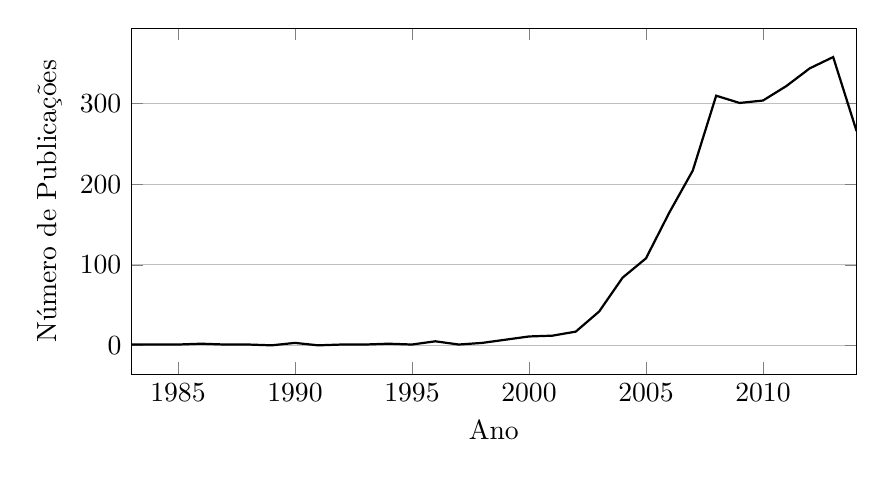
\begin{tikzpicture}
     \begin{axis}[
         xlabel={Ano},
         ylabel={N\'{u}mero de Publica\c{c}\~{o}es},
         width=0.5\paperwidth, height=170,
         xmin=1983,
         xmax=2014,
         ymajorgrids,
         /pgf/number format/.cd,
			use comma,
			1000 sep={}
         ]
      
         \addplot[
			thick,
			black]
%             table [col sep=comma] {scopusStream.dat};
			coordinates {
				(1983,1)
				(1984,1)
				(1985,1)
				(1986,2)
				(1987,1)
				(1988,1)
				(1989,0)
				(1990,3)
				(1991,0)
				(1992,1)
				(1993,1)
				(1994,2)
				(1995,1)
				(1996,5)
				(1997,1)
				(1998,3)
				(1999,7)
				(2000,11)
				(2001,12)
				(2002,17)
				(2003,42)
				(2004,84)
				(2005,108)
				(2006,165)
				(2007,217)
				(2008,310)
				(2009,301)
				(2010,304)
				(2011,322)
				(2012,344)
				(2013,358)
				(2014,266)};
      
     \end{axis}
     \end{tikzpicture}
 
%\end{document}

%	\caption{Progressão anual do número de publicações em inglês, artigos e conferências, considerando o resultado de busca realizada na base Scopus, em 14 de junho de 2016, pela combinação dos termos \emph{learning}/\emph{mining} e \emph{data streams}/\emph{streaming data}
%		%string:
%		%(TITLE-ABS-KEY("mining") AND TITLE-ABS-KEY("data stream")) OR(TITLE-ABS-KEY("mining") AND TITLE-ABS-KEY("streaming data")) OR(TITLE-ABS-KEY("learning") AND TITLE-ABS-KEY("data stream")) OR(TITLE-ABS-KEY("learning") AND TITLE-ABS-KEY("streaming data")) AND ( LIMIT-TO(LANGUAGE,"English" ) ) AND ( LIMIT-TO(DOCTYPE,"cp" ) OR LIMIT-TO(DOCTYPE,"ar" ) )
%	}
%	\label{Fig:scopusStream}
%\end{figure}
%Desde a última década, surgem cada vez mais métodos diferentes que aplicam processo de aprendizagem em fluxos de dados. Esses métodos seguem, principalmente, abordagens supervisionadas (que realizam a extração de conhecimento pelo desenvolvimento de um modelo geral baseado em conjuntos de dados que possuem um atributo especial, chamado classe, que representa o conceito que se deseja aprender) e não supervisionadas (processo capaz de realizar aprendizagem a partir de um conjunto de dados onde a informação de classes não está disponível).
%
%Também nesse período, cresceram os esforços para investigação de métodos de aprendizado semissupervisionado, especialmente em conjuntos de dados clássicos, i.e.,não contínuos. A motivação principal para utilização de métodos de aprendizado semissupervisionado é a disponibilidade de grandes volumes de dados em diversas áreas do conhecimento e o alto custo de interpretação e rotulação (atribuição de classe) manual desses dados. Métodos semissupervisionados consideram tanto um pequeno conjunto de dados rotulados, que possuem informação sobre classe, quanto um grande conjunto de dados não rotulados, que não possuem informação sobre classe, para realizar o processo de aprendizagem, obtendo resultados mais interessantes do que se realizasse o aprendizado exclusivamente pelo pequeno conjunto de dados rotulados ou pelo grande conjunto de dados não rotulados.
%
%Em algumas aplicações de Fluxo Contínuo de Dados, é possível que não haja a totalidade de dados rotulados, ou que apenas um conjunto inicial do fluxo possua rótulos. Mais recentemente, métodos de aprendizado semissupervisionado vê sendo adaptados para a incorporação de mecanismos capazes de lidar com as características de Fluxo Contínuo de Dados.
%
%\section{Motivação e Objetivos}
%
%As vantagens da utilização de métodos de aprendizado semissupervisionado já foram evidenciadas em trabalhos anteriores \cite{Lopes2011,Lopes2012}. O estudo realizado para combinação de agrupamento semissupervisionado com sistemas baseados em regras \emph{fuzzy} propiciou a continuação das investigações que, finalmente, deu origem à proposta apresentada neste documento.
%
%O aprendizado em Fluxos Contínuos de Dados é uma tendência dentro das pesquisas na área de Aprendizado de Máquina, constituindo um tópico promissor para futuras pesquisas, em função do grande interesse observado nos últimos anos, devido à necessidade de aquisição de conhecimento em domínios de características específicas.
%
%O objetivo do trabalho proposto aqui é a investigação de técnicas de aprendizado semissupervisionado aplicados ao contexto de Fluxo Contínuo de Dados. Para tanto, são caracterizados neste documento alguns conceitos inicias sobre aprendizado em  conjunto clássicos e com dados de fluxo contínuo, estudando algumas das principais características dentro desta segunda área. Também é apresentado um conjunto de métodos conhecidos e diferenciados dentro do aprendizado em Fluxo Contínuo de Dados, a fim proporcionar uma visão geral das abordagens que vêm sendo utilizadas.
%
%O levantamento bibliográfico realizado serve de base para a proposta de trabalho para tese de doutoramento, ambos apresentados neste documento.
%
%\section{Organização}
%
%O restante deste documento está estruturado como segue:
%\begin{description}
%\item[Capítulo \ref{chConceitos} - Conceitos Iniciais:] Este capítulo descreve conceitos básicos a respeito de aprendizado supervisionado, não supervisionado e semissupervisionado. É colocada uma caracterização do domínio de aplicações baseadas em Fluxos Contínuos de Dados, além de conceitos iniciais particulares ao Aprendizado de Máquina realizado nessa área e algumas noções básicas que fundamentaram o desenvolvimento de métodos para o aprendizado com dados de fluxo contínuo.
%\item[Capítulo \ref{chRevisao} - Abordagens para Aprendizado em Fluxos Contínuos de Dados:] Após a contextualização apresentada no capítulo anterior, este capítulo traz uma revisão bibliográfica a fim de traçar uma visão geral do estado-da-arte da área de aprendizado em Fluxos Contínuos de Dados. Os métodos que realizam aprendizado semissupervisionado são de particular interesse para este trabalho.
%\item[Capítulo \ref{chProposta} - Proposta de Trabalho] Com base em todo o levantamento e investigações realizadas, parte apresentada neste documento, é apresentada neste capítulo uma proposta de trabalho para a continuação e desenvolvimento de tese dentro da área de aprendizado semissupervisionado com dados de fluxo contínuo.
%\end{description}